\documentclass[tikz,border=10pt]{standalone}
\usepackage{tikz}
\usepackage{verbatim}
\begin{document}
	\usetikzlibrary{arrows,positioning} 
	\tikzset{
		%Define standard arrow tip
		>=stealth',
		% Define arrow style
		pil/.style={
			->,
			thick,
			shorten <=2pt,
			shorten >=2pt,}
	}
	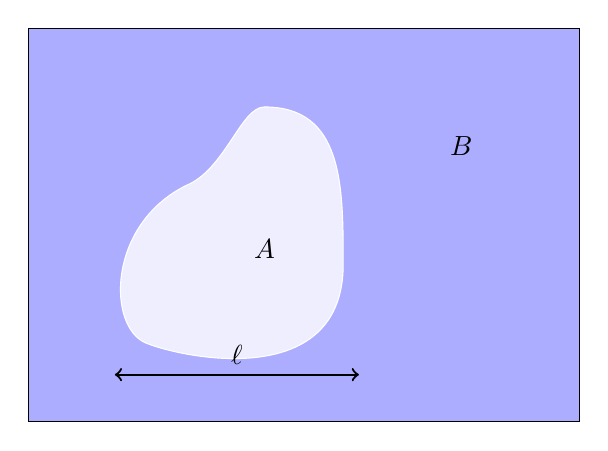
\begin{tikzpicture}
	\tikzstyle{Filling} = [fill=blue!40,fill opacity=0.8]
	\filldraw[Filling]  (0,0)--(0,5)--(7,5)--(7,0)--cycle;
	\filldraw[white, fill opacity= 0.8]  (1.5,1)..controls(2,0.8)and(4,0.4)..(4,2)..controls(4,3)and(4,4)..(3,4)..controls(2.7,4)and(2.5,3.2)..(2,3)..controls
	(1,2.5)and(1.0,1.2)..(1.5,1)--cycle;
	\draw (5.5,3.5) node{$B$};
	\draw (3.0,2.2) node{$A$};
	\draw[<->,thick] (1.1,0.6)--(4.2,0.6);
	\draw (2.65,0.6) node[anchor=south] {$\ell$};
	\end{tikzpicture}
\end{document}